\chapter{Preliminaries}

\label{chapter:preliminaries}
\section{Homogenous coordinate systems}

Homogenous coordinates are a tool to simplify certain geometrical operations by adding an extra dimension.
For example, the general scaling, rotation and translation is expressed in non-homogenous coordinates as:
% To transform a point $m=(u, v)^\top$ from cartesian coordinates to homogenous, simply append $1$ as the third coordinate: $m=(u, v, 1)^\top$.

\begin{equation}
    \vec{m}_1 = 
    \pmb{\mathsf{S}} \pmb{\mathsf{R}}
    \vec{m}_0
    + \vec{t},
\end{equation}

\begin{equation}
    \pmb{\mathsf{S}} = \begin{bmatrix} s_x & 0 \\ 0 & s_y \end{bmatrix}, \pmb{\mathsf{R}} = \begin{bmatrix} \cos(\theta) & -\sin(\theta) \\ \sin(\theta) & \cos(\theta) \end{bmatrix}, \vec{t} = \begin{bmatrix} t_x \\ t_y \end{bmatrix},
\end{equation}

where $m_0$ is the original point,
$m_1$ is the transformed point,
$\pmb{\mathsf{S}}$ is a scaling matrix,
$\pmb{\mathsf{R}}$ is a rotation matrix and 
$\vec{t}$ is a translation vector.

The same operations can be expressed in a homogenous coordinate system using one matrix multiplication as

\begin{equation}
    \begin{bmatrix} \vec{m}_1 \\ 1 \end{bmatrix} = 
    \pmb{\mathsf{S}}_H \pmb{\mathsf{R}}_H \pmb{\mathsf{T}}_H
    \begin{bmatrix} \vec{m}_0 \\ 1 \end{bmatrix},
\end{equation}
\begin{equation}
    \pmb{\mathsf{S}}_H = \begin{bmatrix} s_x & 0 & 1\\ 0 & s_y & 1 \\ 0 & 0 & 1\end{bmatrix}, \pmb{\mathsf{R}}_H = \begin{bmatrix} \cos(\theta) & -\sin(\theta) & 0 \\ \sin(\theta) & \cos(\theta) & 0 \\ 0 & 0 & 1 \end{bmatrix}, \pmb{\mathsf{T}}_H = \begin{bmatrix} 1 & 0 & t_x\\ 0 & 1 & t_y \\ 0 & 0 & 1 \end{bmatrix} ,
\end{equation}
where $\pmb{\mathsf{S}}_H, \pmb{\mathsf{R}}_H$ and $\pmb{\mathsf{T}}_H$ are homogenous transformation matrices.

So in the homogenous coordinate system, all 2D transformations can be combined and expressed as matrix multiplications.

% \subsection{Vanishing point}
% \begin{figure}[h]
%     \centering
%     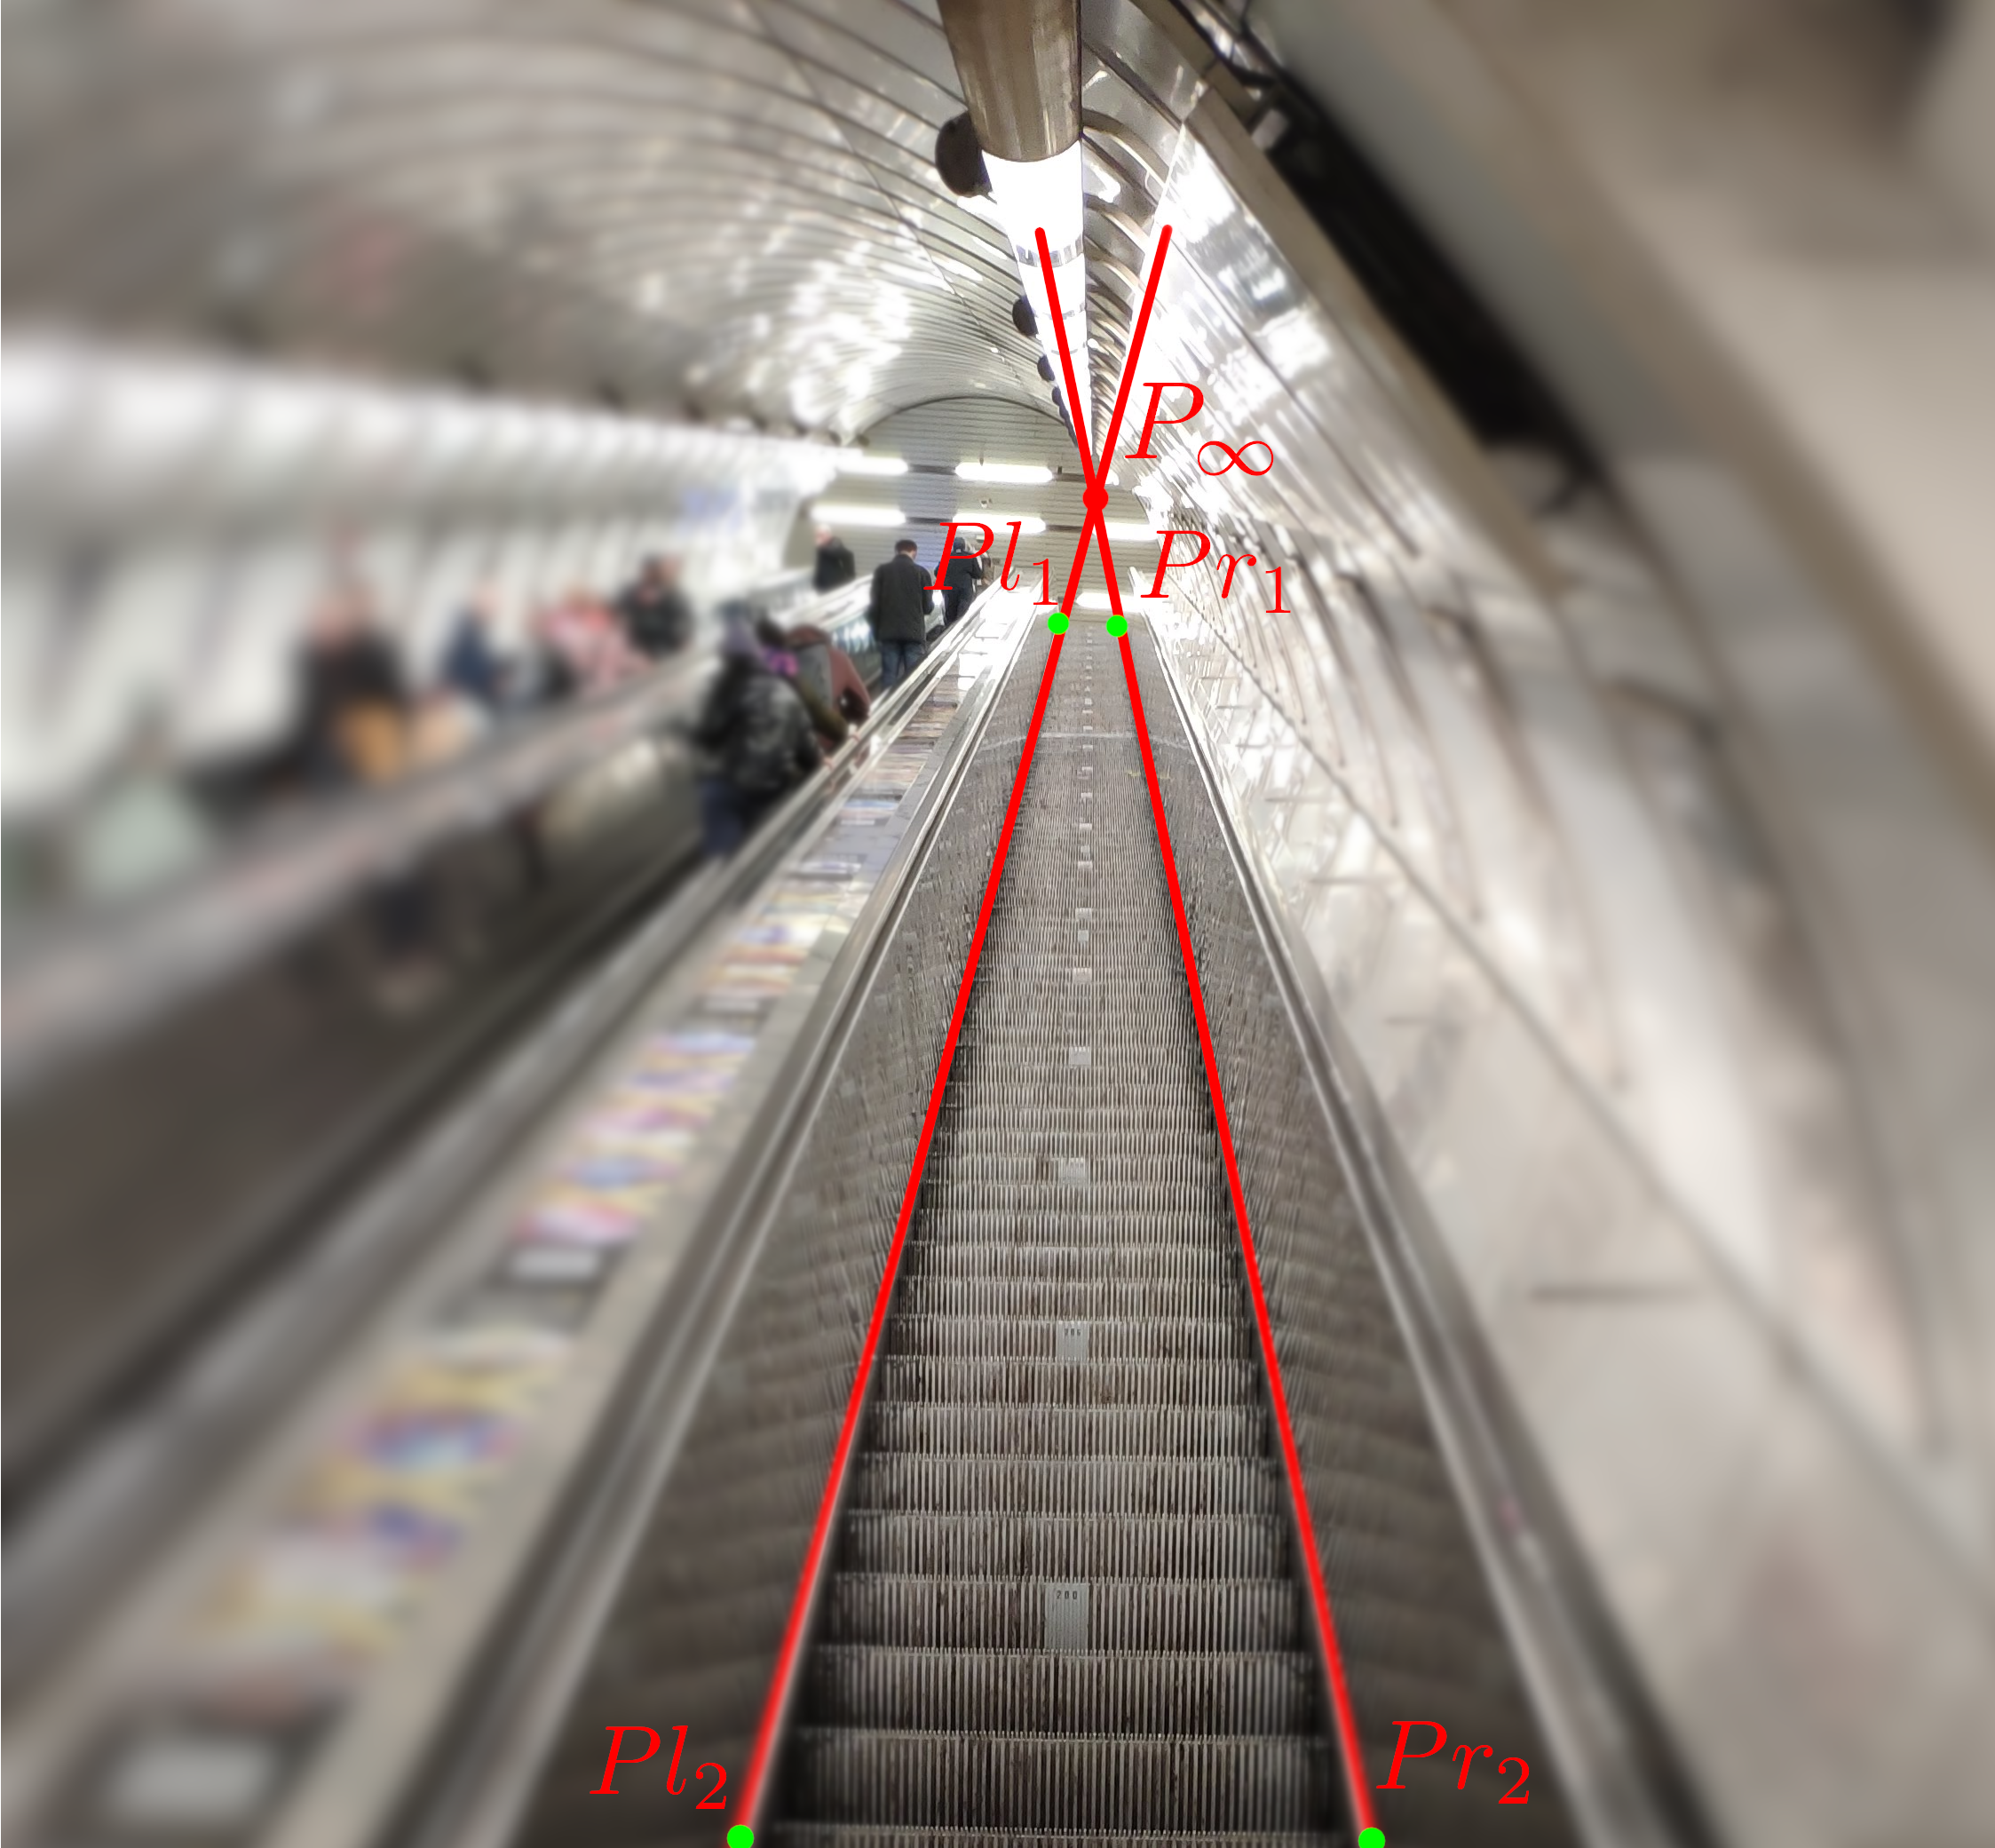
\includegraphics[width=0.75\textwidth]{graphics/parallel_intersection.png}
%     \caption{Parallel lines intersection}
%     \label{fig:intersection_parallel}
% \end{figure}

% \begin{figure}[h]
%     \centering
%     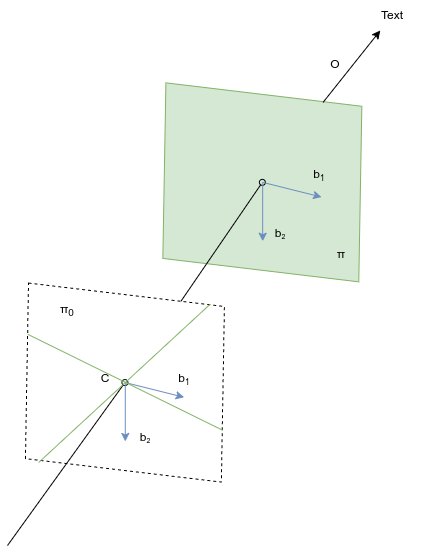
\includegraphics[width=.5\textwidth]{graphics/homogenous.png}
%     \caption{Scheme of homogenous coordinates}
%     \label{fig:homogenous}
% \end{figure}

% In Euclidian geometry, parallel lines are the lines that have no intersection point. 
% In projective geometry, parallel lines intersect at a point $x$ at infinity. 

% In the image \autoref{fig:intersection_parallel} let $l_r$ be a line defined by$Pr_1$ and $Pr_2$, and $l_l$ be a line defined by $Pl_1$ and $Pl_2$. 
% In the 3D world, lines $\vec{l}_l \parallel \vec{l}_r$, but after projection on the image plane $\pi$, lines are interesting at a point $P_\infty$.
% In a general cases, such a point can be computed as a cross product of two parallel lines. 

% Both line and point in a homogenous coordinates are expressed as vectors of three numbers: a homogenous point $\vec{m} = (x, y, z)^\top$ is $\vec{m} = (\frac{x}{z}, \frac{y}{z})^\top$, and a line $\vec{l} = (a, b, c)^\top$, where $a, b, c$ are parameters of a line equation $ax + by + c = 0$. 
% In general case, point at infinity is called an \textit{ideal point} and it is not seen on the image, its coordinates can be expressed as $\vec{m}_{\infty} = (u, v, 0)^\top, \{u, v\} \neq 0$.
% Same about line - such line is called \textit{ideal line} and its coordinates are $\vec{l} = (0, 0, c)^\top, c \neq 0$. In algebraic representation, both ideal point and line are at the plane $\pi_0$ (\autoref{fig:homogenous}, green lines).

% A vanishing point is an image of the point at infinity.
% All world (4D) parallel lines share the same image vanishing point. On a \autoref{fig:intersection_parallel} a $P_{\infty}$ is an image of two parallel lines' intersection point (which is a point at infinity), so it is also a vanishing point.

\section{Pinhole camera model}
A pinhole camera, the canonical perspective camera model - is a model of a simple camera without any optics.
The first example is the camera Obscura - a dark room with a small hole through which the image from outside is projected on the opposite wall. 
This model can be used to express camera geometry with a field of view angles less than $180^{\circ}$.

\subsection{Camera coordinate system}
\begin{figure}[h]
    \centering
    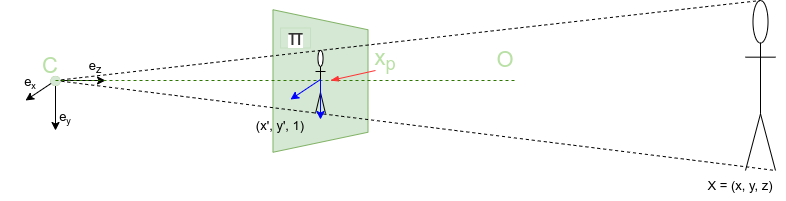
\includegraphics[width=\textwidth]{graphics/td_scene.png}
    \caption{The scheme of a pinhole camera model}
    \label{fig:td_scene_3d}
\end{figure}

\begin{figure}[h]
    \centering
    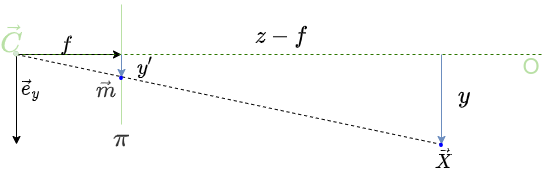
\includegraphics[width=\textwidth]{graphics/td_scene_yz.png}
    \caption{The pinhole camera model, y-z plane}
    \label{fig:td_scene_yz}
\end{figure}

\begin{figure}[h]
  \begin{subfigure}[b]{0.49\textwidth}
    \centering
    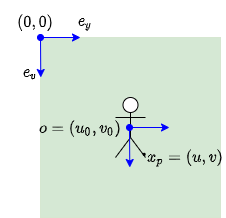
\includegraphics[width=0.74\textwidth]{graphics/td_scene_xy.png}
    \caption{The pinhole camera model, x-y plane}
    \label{fig:td_scene_xy}
  \end{subfigure}
  \hfill
  \begin{subfigure}[b]{0.49\textwidth}
    \centering
    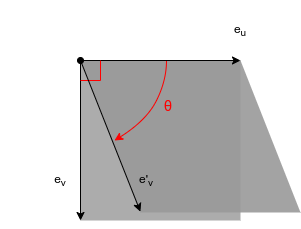
\includegraphics[width=1\textwidth]{graphics/pixel.png}
    \caption{A scheme of a pixel skew}
    \label{fig:Kframes}
  \end{subfigure}
\end{figure}

In the physical implementation of the camera Obscura, the projective plane is on the opposite side from the projection center (or camera center $\vec{C}$ in the pinhole camera model), and the image is reversed and mirrored. 
However, in most computer vision literature, authors assume that it is on the same side as the object (see \autoref{fig:td_scene_3d}).
In \autoref{fig:td_scene_3d} a camera with camera center $C$ in a coordinate system with origin at $\vec{C}$ and basis vectors $(\vec{e}_x, \vec{e}_y, \vec{e}_z)$ is observing human. 
Each point $\vec{X} = (x, y, z)^\top$ in a world coordinate system has a projection $\vec{m} = (u, v)^\top$ on a plane $\pi$ which is located on a distance $f$ from the camera center (\autoref{fig:td_scene_yz}). 
The optical axis $\vec{O}$ is a ray perpendicular to plane $\pi$, and on the image the point $ \vec{O} \cap \pi = \vec{o}$ is the center of the image, see \autoref{fig:td_scene_xy}.

\subsection{Camera matrix}
The camera calibration matrix is a matrix that includes the camera's \textit{intrinsic} parameters - focal length, pixel skew angle ($\theta$), as on \autoref{fig:Kframes}, pixel aspect ratio \textit{a} and principle point coordinates $\vec{o} = (u_0, v_0)$ \autoref{fig:td_scene_xy}.
\begin{equation}
    \mat{K} = \begin{bmatrix}
        f_x & -a f \cot(\theta) & u_0 \\
        0 & f_y & v_0 \\
        0 & 0 & 1 \\
    \end{bmatrix} 
    \textrm{ ,units: } [f]=m, [u_0]=px, [v_0]=px, [a]=1,
\end{equation}

where $f_x = af$, $f_y = \frac{f}{\sin{\theta}}$, $f$ is a focal length used to convert world length ratios to pixels.

Most modern digital cameras have no skew and square pixels, so in most cases, the camera matrix can be simplified to:

\begin{equation}
    \label{eq:kmat}
    \pmb{\mathsf{K}} = \begin{bmatrix}
        f_x & 0 & u_0 \\
        0 & f_y & v_0 \\
        0 & 0 & 1 \\
    \end{bmatrix};
\end{equation}

\subsection{Projection matrix}

\begin{figure}[h]
    \centering
    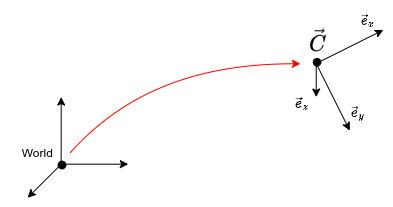
\includegraphics[width=.5\textwidth]{graphics/frames.png}
    \caption{Transformation from world to camera coordinate frames}
    \label{fig:frames}
\end{figure}

To translate a point from a world coordinate frame to an image coordinate frame, the Image projection matrix $\pmb{\mathsf{P}}$ is used. 
The canonical projection matrix $\pmb{\mathsf{P}}_0$ assumes that the camera is in the world coordinate center and that the calibration matrix $\pmb{\mathsf{K}} = \pmb{\mathsf{I}}$
\begin{equation}
\pmb{\mathsf{P}}_0 = \begin{bmatrix} \pmb{\mathsf{I}} & | & \vec{0} \end{bmatrix} = 
    \begin{bmatrix}
    1 & 0 & 0 & 0 \\
    0 & 1 & 0 & 0 \\
    0 & 0 & 1 & 0 \\
    \end{bmatrix};
\end{equation}

However, this case is impractical. 
The canonical projection matrix is not used in practice because each real camera is different. 
Instead, the image projection matrix $\mat{P}$ is used with a camera matrix $\mat{K}$ to transform canonical $\mat{P}_0$ to perspective $\mat{P}$:

\begin{equation}
\pmb{\mathsf{P}} = \pmb{\mathsf{K}} \begin{bmatrix} \pmb{\mathsf{I}} & | & \vec{0} \end{bmatrix} = 
    \begin{bmatrix} 
    f_x & 0 & u_0 & 0 \\
    0 & f_y & v_0 & 0 \\ 
    0 & 0 & 1 & 0 \\
    \end{bmatrix}.
\end{equation}

The world coordinate center is usually not located at point $\vec{C}$ (\autoref{fig:frames}). 
It may be rotated using a rotation matrix $\mat{R}$ and translated on vector $\vec{t}$ where $\mat{R}$ is a $3x3$ matrix with $det(\mat{R}) = 1$ and $\mat{R}^{-1} = \mat{R}^\top$. 
Therefor, in the general case the projection can be expressed as
\begin{equation}
    \label{eq:PKRt}
    \pmb{\mathsf{P}} = \pmb{\mathsf{K}} \begin{bmatrix} \pmb{\mathsf{R}} & | & \vec{t} \end{bmatrix} = 
    \pmb{\mathsf{K}} \begin{bmatrix} \pmb{\mathsf{R}} & | & - \pmb{\mathsf{R}} \pmb{\mathsf{C}} \end{bmatrix},
\end{equation}

where $\vec{C}$ is the camera's position in a world reference frame. 

Image point $\vec{m} = (u, v)^\top$ can be obtained from a 3D point $\vec{X}$ using the projection matrix $\mat{P}$ as

\begin{equation}
    \label{eq:projection}
    \lambda \begin{bmatrix} 
        u \\ v \\ 1 \end{bmatrix} = \pmb{\mathsf{P}} \begin{bmatrix} x \\ y \\ z \\ 1
    \end{bmatrix},
\end{equation}

\begin{equation}
    \label{eq:proj_min}
    \lambda 
    \begin{bmatrix} 
    \vec{m} \\ 1 \end{bmatrix} = \pmb{\mathsf{P}} \begin{bmatrix} \vec{X} \\ 1
    \end{bmatrix},
\end{equation}
where $\lambda \neq 0$ is a free scaling parameter.

\subsection{Skew-symmetric 3x3 matrix}
A skew-symmetric or antisymetric matrix of vector $\vec{b} = (b_1, b_2, b_3)^\top$ is defined as
\begin{equation}
    [\vec{b}]_{\times} = \begin{bmatrix}
        0 & -b_3 & b_2 \\ 
        b_3 & 0 & b_1 \\ 
        -b_2 & b_1 & 0 \\ 
    \end{bmatrix}.
\end{equation}

This matrix has several useful properties, but the most important in this thesis is that it generalizes a cross product as matrix multiplication:
\begin{equation}
    \vec{a} \times \vec{b} = [\vec{a}]_{\times} \vec{b}.
\end{equation}
The notation is taken from \cite{hartley_zisserman_2004}, p. 581.

\section{Epipolar geometry}
\label{sec:epipolar_geometry}
\begin{figure}[h]
    \centering
    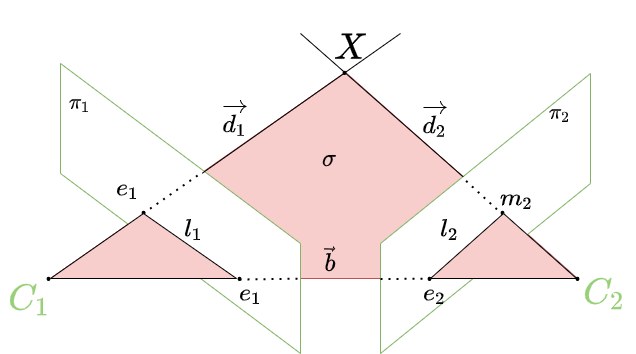
\includegraphics[width=\textwidth]{graphics/epipolar.png}
    \caption{A scheme of epipolar geometry}
    \label{fig:epipolar_std}
\end{figure}

\autoref{fig:epipolar_std} shows a scheme of two cameras with different camera centers $\vec{C}_1$ and $\vec{C}_2$ connected with a base vector $\vec{b} = \vec{C}_2 - \vec{C}_1$. 
Both of the cameras observe a 3D point $X$. 
Projections of this point to $\pi_1$ and $\pi_2$ are $\vec{m}_1$ and $\vec{m}_2$ respectivly. 
Points $\vec{C}_1, \vec{C}_2$ and $\vec{X}$ form an \textit{epipolar plane} $\sigma$.
The lines $\sigma \cap \pi_1 = l_1$ and $\sigma \cap \pi_2 = l_2$ are \textit{epipolar lines}. 
The epipolar line $l_1$ passes through an \textit{epipole} $\vec{e}_1$ and through point $\vec{m_1}$, where $\lambda [\vec{e}_1 | 1]^\top = \mat{P}_1 \vec{C}_2$
Similarly, line $l_2$ passes through an \textit{epipole} $\vec{e}_2$ and through point $\vec{m_2}$, where $\lambda [\vec{e}_2 | 1]^\top = \mat{P}_2 \vec{C}_1$.

\subsection{The epipolar constraint}
Having a set of two cameras the relationship between them and the constraints on them can be expressed by two matrices: the \textit{essential matrix} $\pmb{\mathsf{E}} \in \mathbb{R}^{3x3},( rank(\mat{E}) = 2)$, and the \textit{fundamental matrix} $\mat{F} \in \mathbb{R}^{3x3}, (rank(\mat{F}) = 2)$. Matrix $\mat{E}$ is obtained as
\begin{equation}
    \label{eq:E}
    \pmb{\mathsf{E}} = \pmb{\mathsf{R}}_2 [\vec{C}_2 - \vec{C}_1]_{\times} \pmb{\mathsf{R}}_1^\top = [-\vec{t}_{21}]_{\times} \pmb{\mathsf{R}}_{21} = [\vec{b}]_{\times} \pmb{\mathsf{R}}_{21},
\end{equation}
and matrix $\mat{F}$ as
\begin{equation}
    \label{eq:F}
    \pmb{\mathsf{F}} = \pmb{\mathsf{K}}_2^{-T} \pmb{\mathsf{R}}_2 [\vec{C}_2 - \vec{C}_1]_{\times} \pmb{\mathsf{R}}_1^\top \pmb{\mathsf{K}}_1^{-1} = 
    \pmb{\mathsf{K}}_2^{-T} [-\vec{t}_{21}]_{\times} \pmb{\mathsf{R}}_{21} \pmb{\mathsf{K}}_1^{-1} = 
    \pmb{\mathsf{K}}_2^{-T} \pmb{\mathsf{E}} \pmb{\mathsf{K}}_1^{-1},
\end{equation}
where 
$\mat{R}_{21} = \mat{R}_2 \mat{R}_1^\top$ is a relative camera rotation and 
$\vec{t}_{21} = -\mat{R}_2 \vec{b} = \vec{t}_2 - \mat{R}_{21}\vec{t}_1$ is a relative camera translation.

An algebraic expression of the important properties of matrix $F$ using notation from \autoref{sec:epipolar_geometry} are:
\begin{equation}
    \label{eq:Fm2}
    \lambda l_1 = \pmb{\mathsf{F}}^\top \begin{bmatrix} \vec{m}_2 \\ 1 \end{bmatrix},
\end{equation}
\begin{equation}
    \label{eq:Fm1}
    \lambda l_2 = \pmb{\mathsf{F}} \begin{bmatrix} \vec{m}_1 \\ 1 \end{bmatrix},
\end{equation}
\begin{equation}
    \label{eq:fefe}
    \pmb{\mathsf{F}} \begin{bmatrix} \vec{e}_1 \\ 1 \end{bmatrix} = \pmb{\mathsf{F}}^\top \begin{bmatrix} \vec{e}_2 \\ 1 \end{bmatrix} = 0,
\end{equation}
\begin{equation}
    \label{eq:epiconstr}
    \begin{bmatrix} \vec{m}_2 & | & 1 \end{bmatrix} \pmb{\mathsf{F}} \begin{bmatrix} \vec{m}_1 \\ 1 \end{bmatrix} = 0.
\end{equation}
Matrix $\pmb{\mathsf{F}}$ maps points from $\pi_1$ to epipolar lines on $\pi_2$ and vice versa (\eqref{eq:Fm2} and \eqref{eq:Fm1}); epipoles $\vec{e}_1$ and $\vec{e}_2$ are right and left nullspaces basis vectors of $\pmb{\mathsf{F}}$ respectivly (\eqref{eq:fefe}).
Epipolar constraint \eqref{eq:epiconstr} means that a point and its corespondent line are on the same plane (\eqref{fig:epipolar_std}, plane $\sigma$).

\section{Stereovision}

\begin{figure}[h]
    \centering
    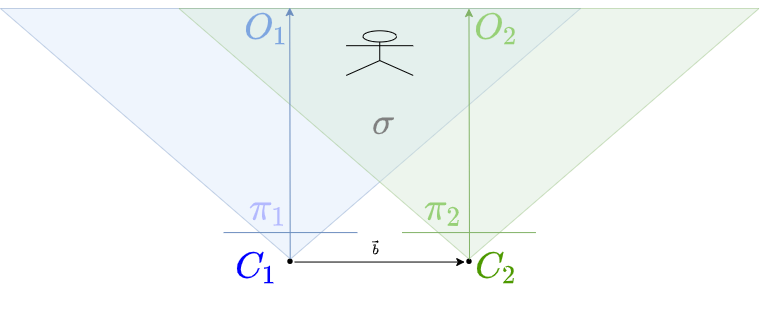
\includegraphics[width=0.8\textwidth]{graphics/stereopair.png}
    \caption{A stereovision scheme}
    \label{fig:sch_stereo}
\end{figure}
\begin{figure}[h]
    \centering
    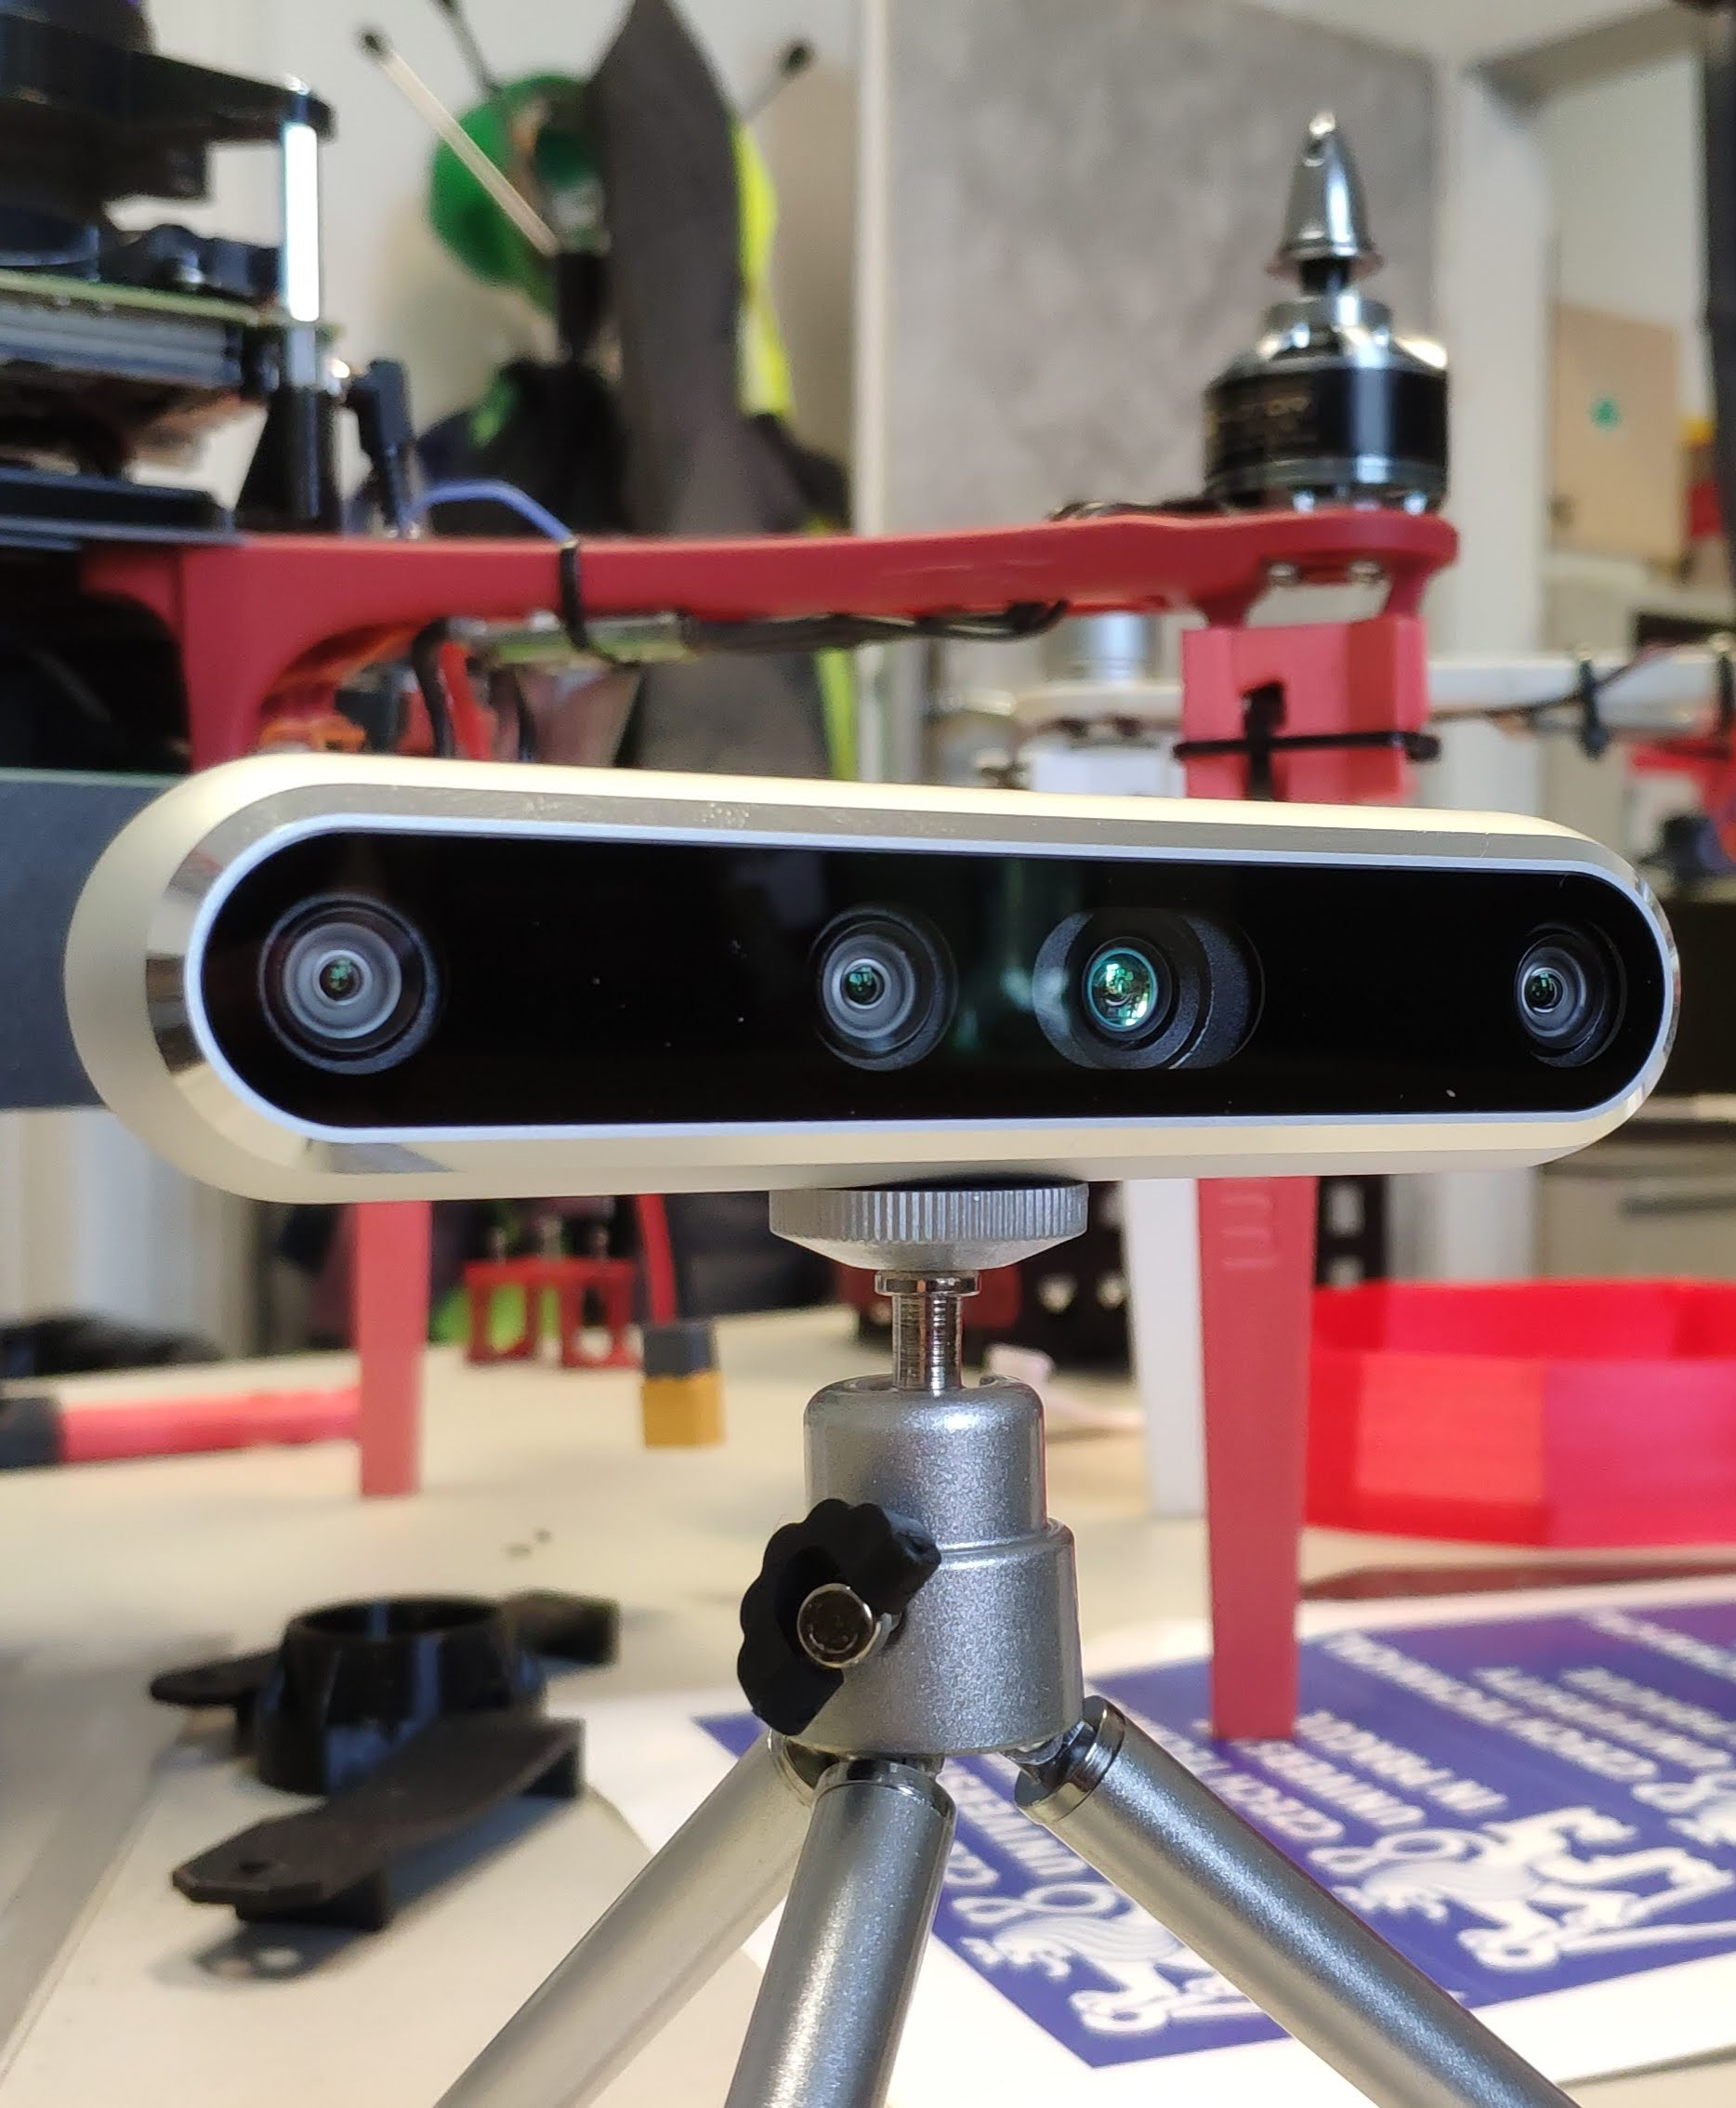
\includegraphics[width=0.3\textwidth]{graphics/stereo_example.jpg}
    \caption{Industrial stereocamera example, Intel Realsense D455}
    \label{fig:stereo_ex}
\end{figure}

% \begin{figure}[h]
%   \begin{subfigure}[b]{0.3\textwidth}
%     \centering
%     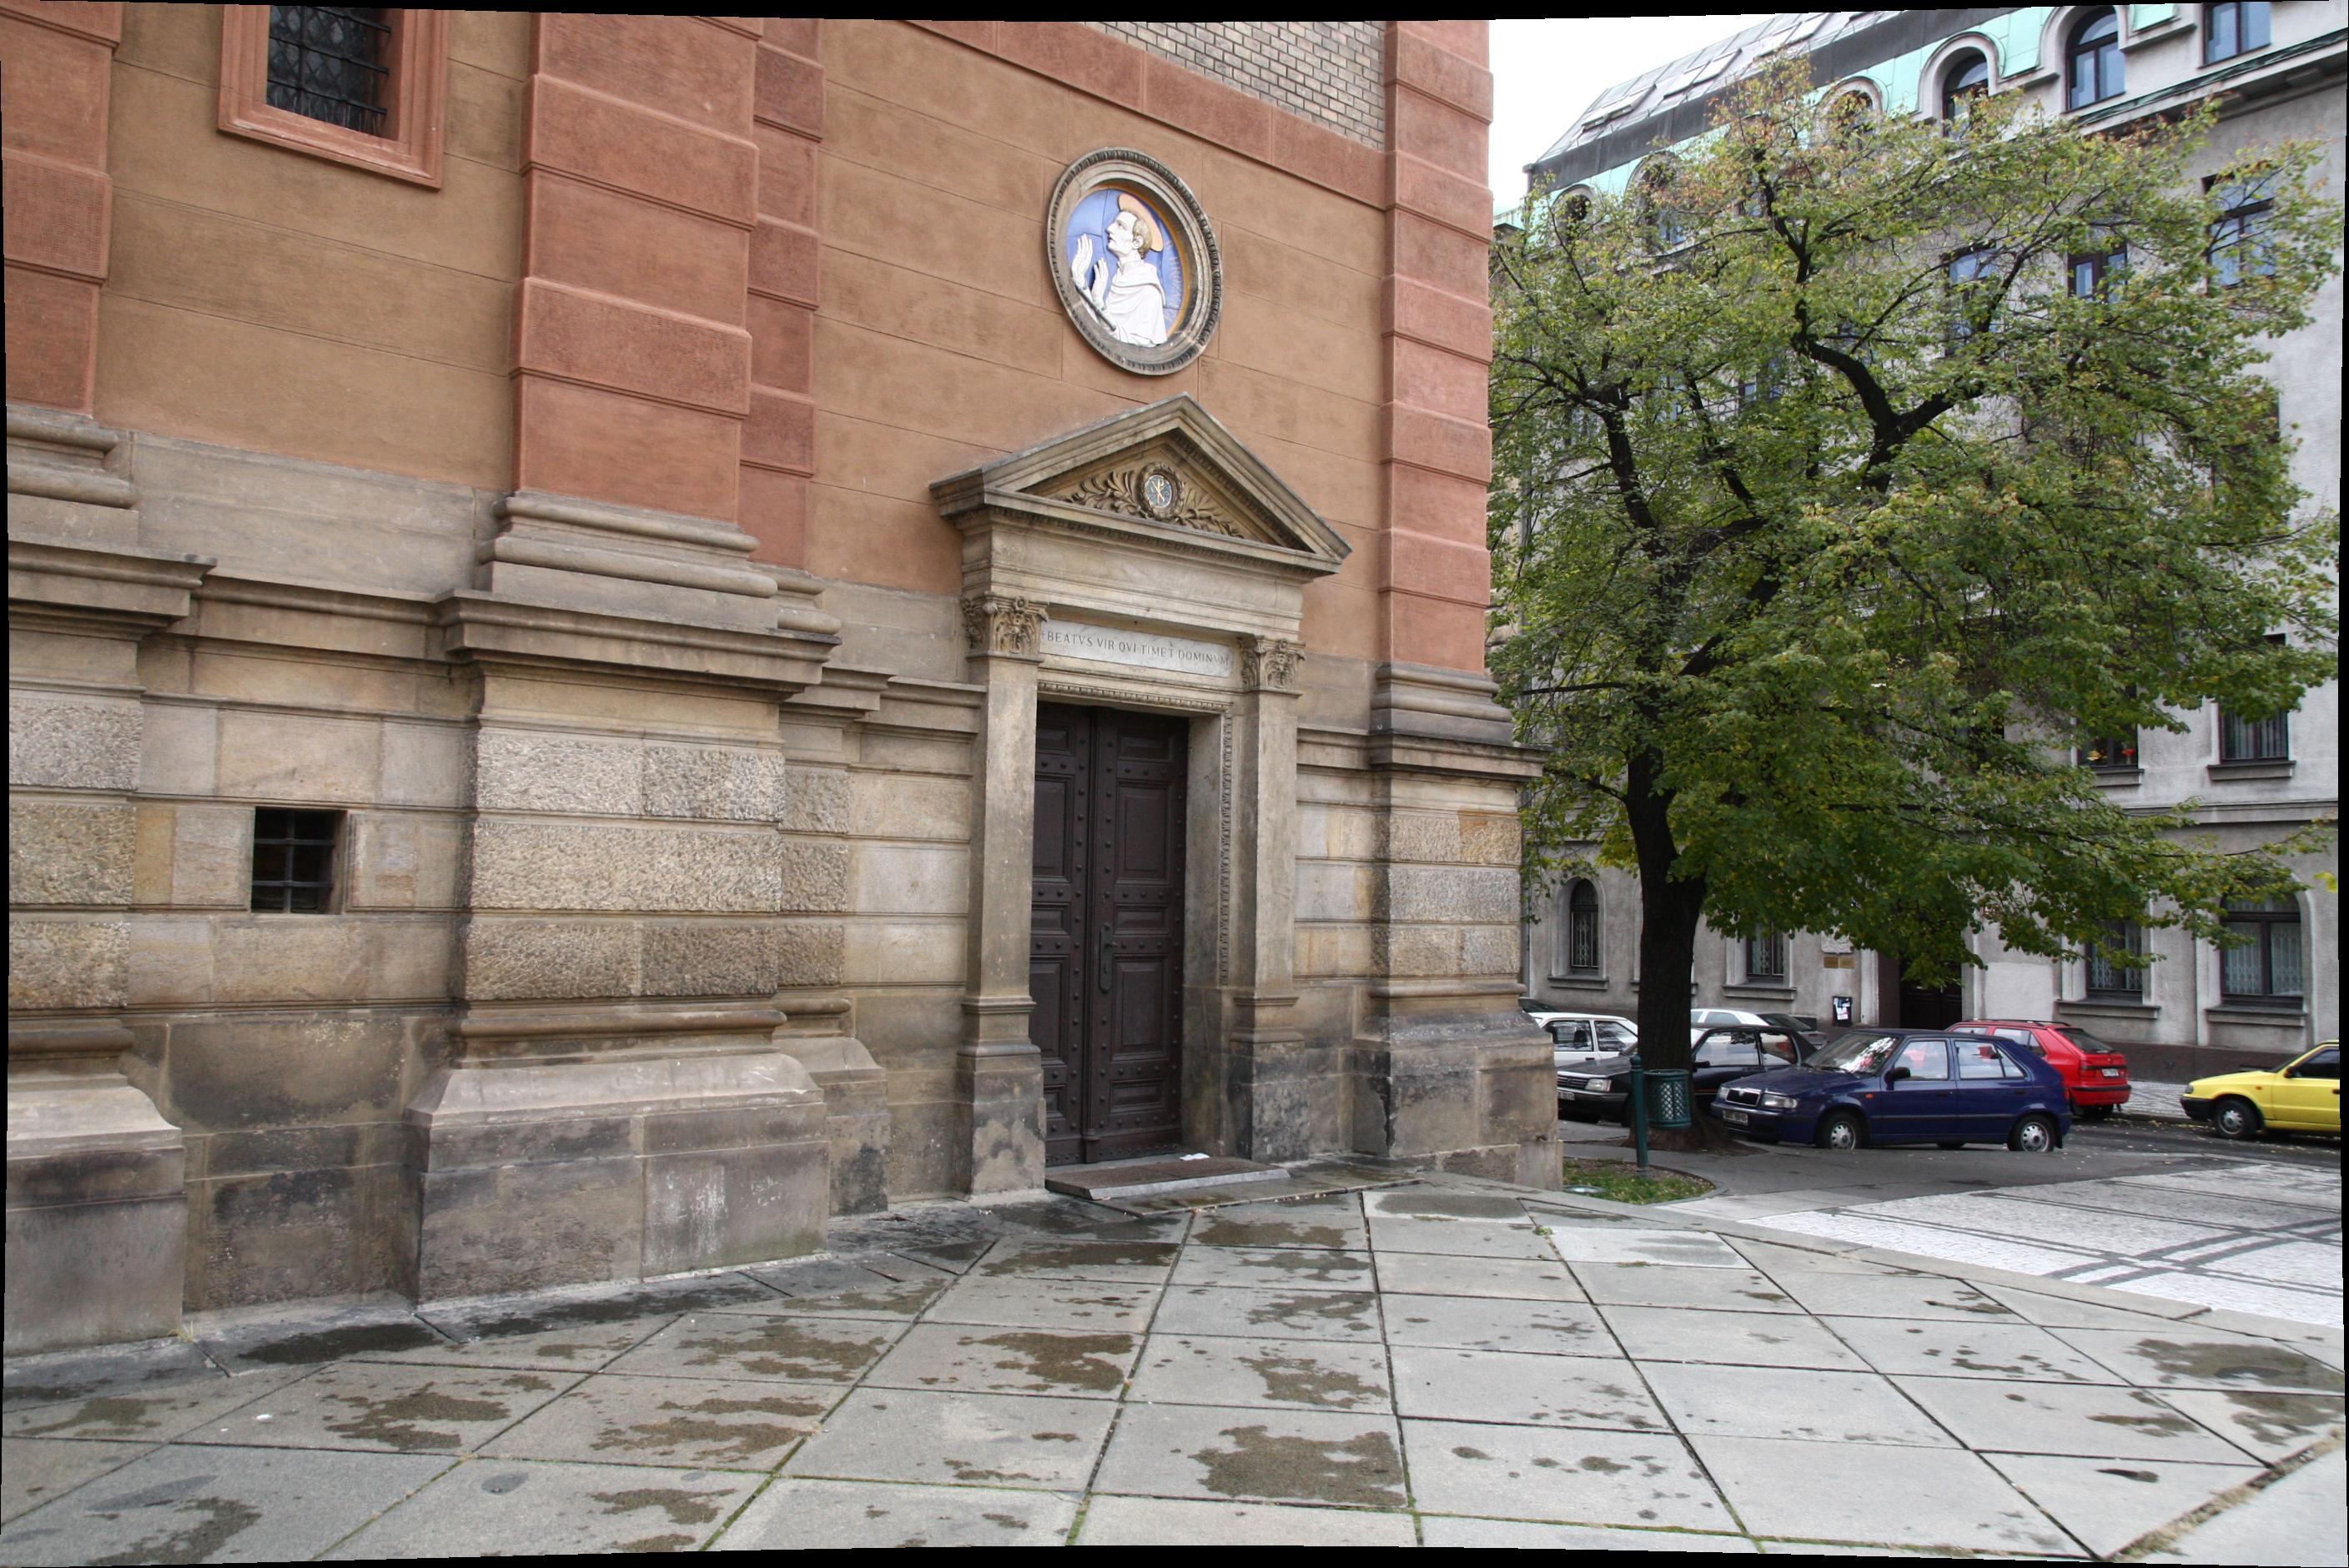
\includegraphics[width=\textwidth]{graphics/01.jpg}
%     \caption{The first image}
%     \label{fig:stereo_1}
%   \end{subfigure}
%   \hfill
%   \begin{subfigure}[b]{0.3\textwidth}
%     \centering
%     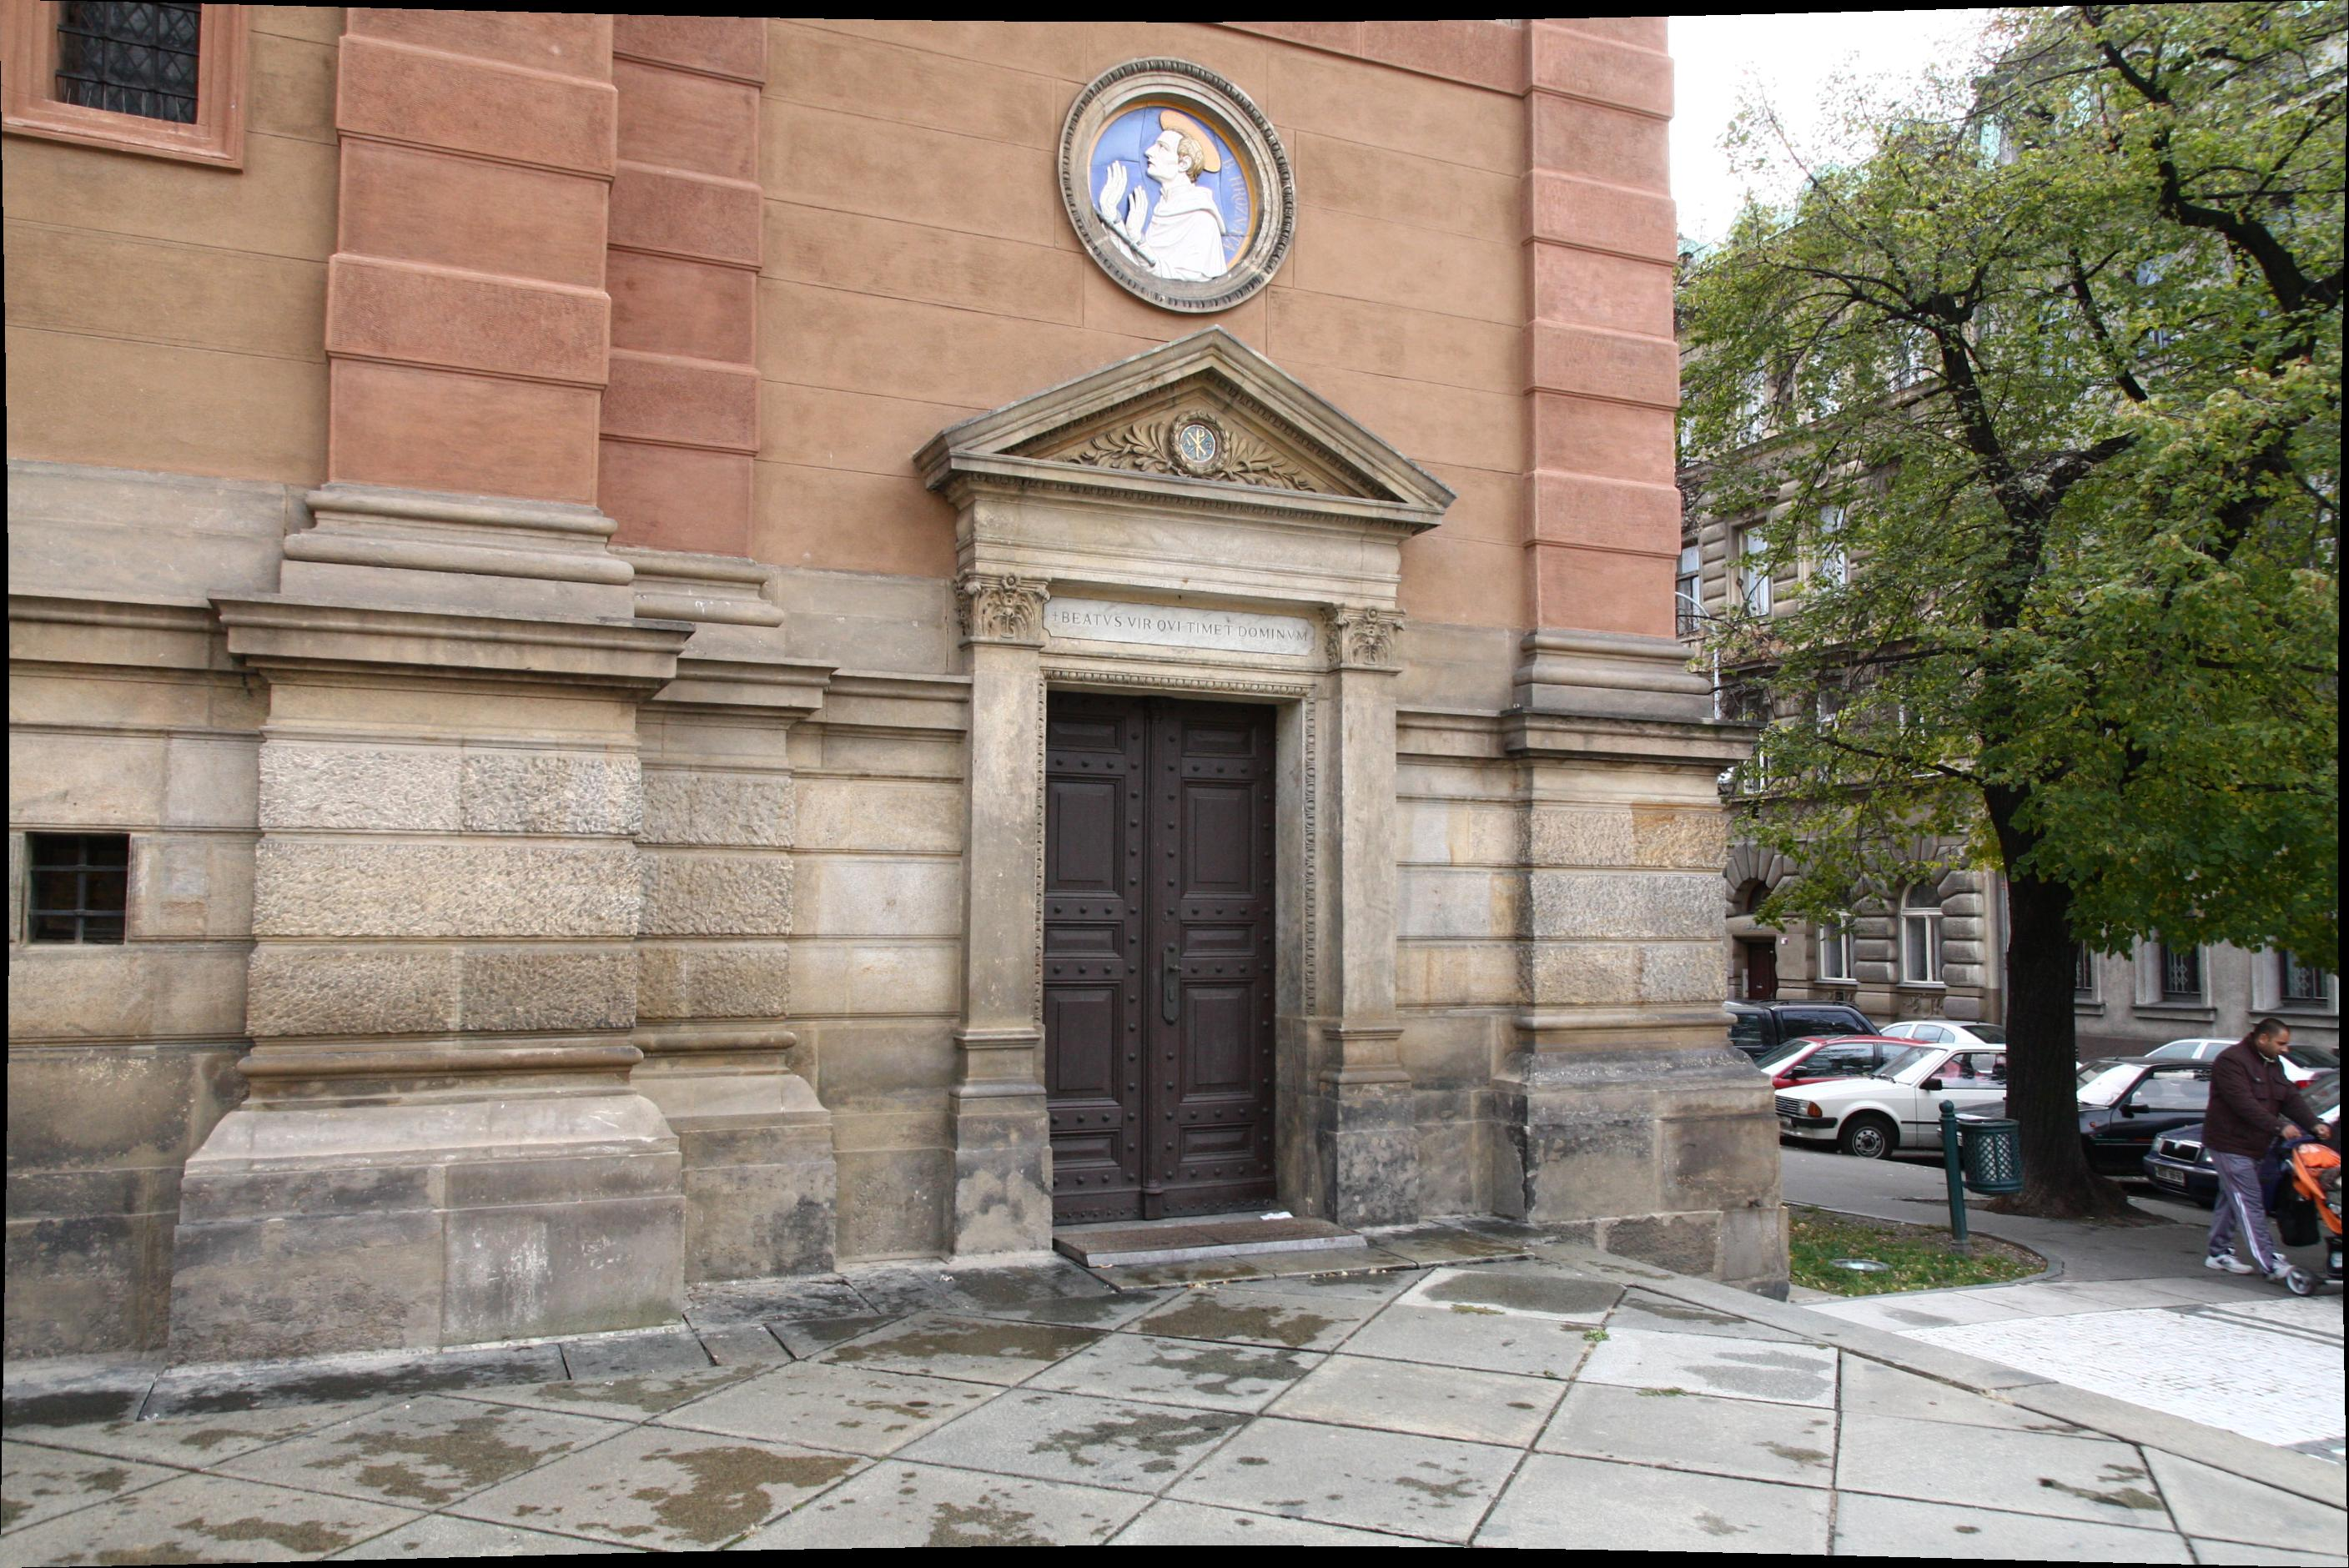
\includegraphics[width=\textwidth]{graphics/02.jpg}
%     \caption{The second image}
%     \label{fig:stereo_2}
%   \end{subfigure}
%   \hfill
%   \begin{subfigure}[b]{0.3\textwidth}
%     \centering
%     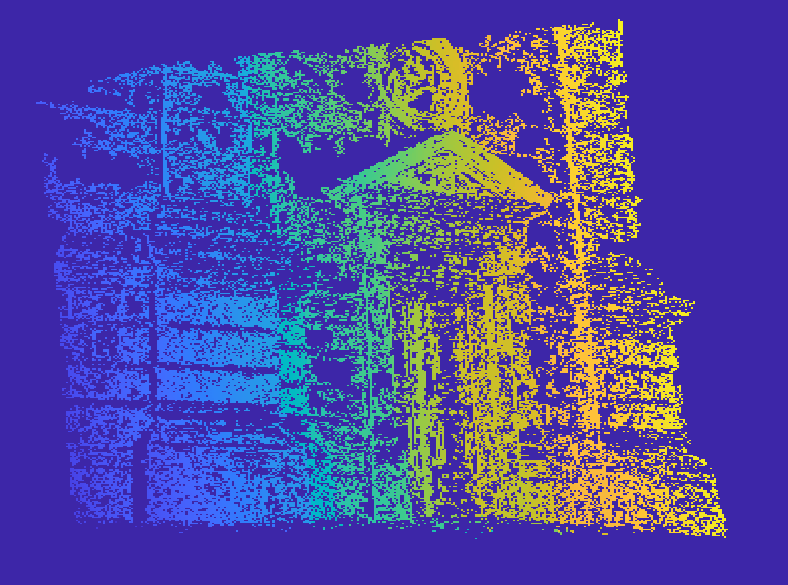
\includegraphics[width=\textwidth]{graphics/disparity.png}
%     \caption{The disparity map}
%     \label{fig:stereo_disp}
%   \end{subfigure}
% \end{figure}

Every digital image has only 2D information about a scene projected onto the image plane as in the \autoref{fig:td_scene_3d}.
Computer stereo vision is a process of extracting a depth image from a pair of images of the same scene. 
The depth maps are then used in SLAM, obstacle avoidance or detailed environment reconstruction in robotics.
In the \autoref{chapter:intro} the most common methods of a depth vision are described, and among them, there are computationally expensive Neural Networks approaches and expensive in terms of money Lidars.
The stereo camera is a tradeoff between price and processing complexity.

Usually, a stereo camera has a pair of cameras located at a distance $||\vec{b}||$ pointing in the same direction, similarly to the human eye (a scheme is in the \autoref{fig:sch_stereo}, and an example of a stereo camera is shown in \autoref{fig:stereo_ex}). 
Sometimes, a fusion of multiple cameras and other sensors can be used: the Intel Realsense shown in \autoref{fig:stereo_ex} has two cameras, a color sensor and an IR projector in case the images have no texture or no feature points was detected.
% The intermediate result of a depth reconstruction is a disparity map computation.
% Disparity map is such a matrix of dimensions $H \times W \times 1$, where $H$ and $W$ are the max height and width of the image pair, and the last channel is a distance of this point, 
% The disparity map from \autoref{fig:stereo_1} and \autoref{fig:stereo_2} is in the \autoref{fig:stereo_disp}.


% It is possible to calculate only the non-zero multiple of $\mat{E}$ from image correspondences so that the scene can be reconstructed only up to a scale, but knowing the translation vector $\vec{b}$ (refer to \autoref{fig:sch_stereo}), the scale can be calculated.

% The corresponding epipolar lines lie on the same image rows ($l_1 = l_2$), and intersect at "points at infinity", which algebraically means
% \begin{equation}
%     \label{eq:e1e2}
%     \vec{e}_1 = \vec{e}_2 = \lambda \begin{bmatrix} 1 \\ 0 \\ 0 \end{bmatrix}.
% \end{equation}
% The epipole is a point of intersecting all epipolar lines, so having the intersecting point ($\vec{e}_1$) and image point, the epipolar line can be calculated as
% \begin{equation}
%     \label{eq:e1m1}
%     \lambda l_1 = \vec{e}_1 \times \begin{bmatrix}
%         \vec{m}_1 \\ 1
%     \end{bmatrix} = [\vec{e}_1]_\times \begin{bmatrix} \vec{m}_1 \\ 1\end{bmatrix},
% \end{equation}
% therefore considering \eqref{eq:Fm1}, \eqref{eq:Fm2}, \eqref{eq:e1e2} and \eqref{eq:e1m1} 

% \begin{equation}
%     \label{eq:F_simple}
%     \pmb{\mathsf{F}} = \lambda [\vec{e}_1]_\times = \lambda \begin{bmatrix}
%         0 & 0 & 0 \\
%         0 & 0 & -1 \\
%         0 & 1 & 0 \\
%     \end{bmatrix}.
% \end{equation}

% Furthermore, let us consider two correspondences $\vec{a}_1 = (u_1, v)^\top$ and $\vec{a}_2 = (u_2, v)^\top $. 
% Having correspondent points on the same row means that the feature matcher can use this correlation to accelerate a matching process.
% It is possible to reconstruct a dense point cloud as in \autoref{fig:pc_output} with this approach.

\section{Reprojection error}
\label{sec:error_reprojection}
In ideal case, when calibration matrix has no error and stereopair position computed precisely, rays $\vec{d}_1$ and $\vec{d}_2$ \autoref{fig:epipolar_std} intersects in a point $\vec{X}$. 
However, calibrations are done with some precision only, so reprojection error is used to measure this precision.

After the 3D pose of a point is computed, to measure its reprojection error, it should be projected back on an image, and a new distance should be computed.

Consider a general projection matrix $\mat{P}_i$ as
\begin{equation}
    \label{eq:p_general}
    \mat{P}_i = \begin{bmatrix} (p_i^1)^\top \\ (p_i^2)^\top \\ (p_i^3)^\top \end{bmatrix},
\end{equation}
the reprojection error is defined as 
\begin{equation}
    e^2(\underline{X}) = \sum_{c=1}^{2}{  
    \begin{bmatrix}
        \begin{pmatrix}
            u_c - \frac{(p_c^1)^\top \underline{X}}{(p_c^3)^\top \underline{X}}
        \end{pmatrix}^2 + 
        \begin{pmatrix}
            v_c - \frac{(p_c^2)^\top \underline{X}}{(p_c^3)^\top \underline{X}}
        \end{pmatrix}^2
    \end{bmatrix}
    },
\end{equation}
where $m_c = \begin{bmatrix} u_c \\ v_c \end{bmatrix}$, $\underline{X} = \begin{bmatrix} \vec{X} \\ 1 \end{bmatrix}$.
